\documentclass[12pt, a4paper]{article}
\usepackage[utf8]{inputenc}
\usepackage{hyperref}
\usepackage{array}
\usepackage{graphicx}
\usepackage{float}

% See here:
% http://tex.stackexchange.com/questions/31186/how-to-move-a-paragraph-to-the-bottom-of-the-page-without-vspace
\newenvironment{bottomPara}{\par\vspace*{\fill}}{\clearpage}

\begin{document}
\title{Brewduino}
\author{
	Andi Anderson
	\and
	Fraser George
	\and
	Adam McGhie
	\and
	Aidan O'Grady
	\and
	Kristine Semjonova
}
\date{}
\maketitle

\begin{figure}[H]
    \centering
    
\includegraphics[height = 6cm]{images/pi-logo}
    
\includegraphics[height = 6cm]{images/arduino-logo}
\end{figure}

\begin{bottomPara}
\noindent \textbf{CS413 Embedded Systems}

\noindent \textbf{Group One}

\noindent \textbf{Phase One Report}

\noindent \textbf{University of Strathclyde, Glasgow}
\newpage

We confirm and declare this report and the assignment work is entirely
the product of our own efforts and we have not used or presented the work of
others herein.\\

% See here: 
% http://tex.stackexchange.com/questions/179184/how-to-make-a-blank-underline
Signature: $\rule{5cm}{0.15mm}$ \hfill Date: $\rule{3cm}{0.15mm}$ \\

Signature: $\rule{5cm}{0.15mm}$ \hfill Date: $\rule{3cm}{0.15mm}$ \\

Signature: $\rule{5cm}{0.15mm}$ \hfill Date: $\rule{3cm}{0.15mm}$ \\

Signature: $\rule{5cm}{0.15mm}$ \hfill Date: $\rule{3cm}{0.15mm}$ \\

Signature: $\rule{5cm}{0.15mm}$ \hfill Date: $\rule{3cm}{0.15mm}$
\end{bottomPara}
\newpage
\tableofcontents
\newpage

% ------------------------------------------------------------------------------
% ------------------------------------------------------------------------------

\section{Introduction}
The initial scope of the assignment is to design and implement an embedded
systems `gadget' with the use of an Arduino and/or a Raspberry Pi.

After a week of discussion, we have decided to implement the Hyper Text 
Coffee Pot Control Protocol (HTCPCP)\cite{HTCPCP}, with a system that allows
the user to send requests for coffee over  internet for either immediate or
future consumption. A server will be implemented to handle the requests to be
sent to our Arduino controlled coffee pot, which will then create coffee on
demand. In addition, we hope to include the functionality of adapting the
Barduino, a project from a previous year, to supply milk or other substances to
a user’s drink as well.
\newpage

% ------------------------------------------------------------------------------
% ------------------------------------------------------------------------------

\section{Assessment of Capabilities}
\subsection{Arduino}
The Arduino is an open source microcontroller primarily aimed at electronics
prototyping. It can interact with various components such as LEDs, motors, etc.
Software can used to utilize these sensors, actuators and other electrical
components, making it a popular product for use in such projects, especially in
education.

As it is a microcontroller it is designed to interact with analogue inputs of
the outside world, which the Raspberry Pi does not have the ability to do as it
can only deal with digital I/O (via GPIO). This allows easy collection of data
through various sensors. 

The Arduino Uno is the microcontroller we have decided to use for this project,
as it meets the requirements for our project, listed below:

\begin{itemize}
	\item Has sufficient size of onboard flash to hold the main program.
	\item Can be easily extended through the use of shields for additional
	hardware interface requirements.
	\item Uses 5V supply, meaning it does not require any power transformers to
	be compatible with other components (i.e. Raspberry Pi).
\end{itemize}

The primary disadvantages of the Arduino when compared to the Raspberry Pi is
it's lack of network capabilities, and the Arduino's lack of processor power.
The Pi allows us to run the necessary independent web server, and make it
accessible to an external client. Due to this the Pi shall be do any
computationally intensive tasks and use the Arduino to interact with the other
hardware.

\begin{figure}[H]
    \centering
    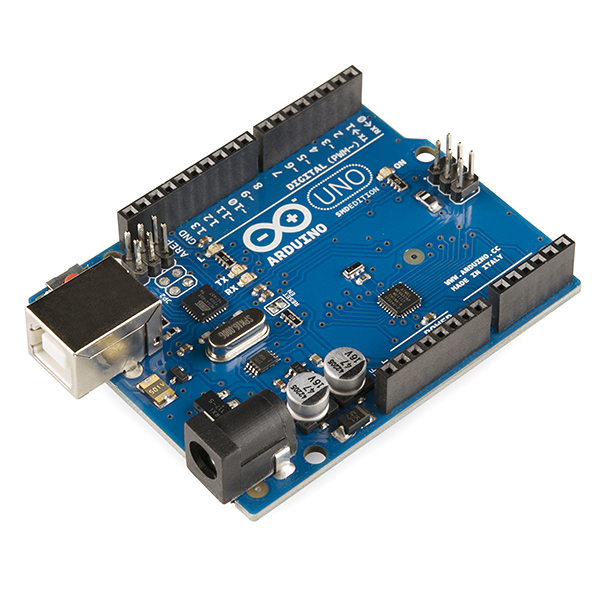
\includegraphics[scale = 0.25]{images/arduino-uno}
    \caption{Arduino Uno.\cite{ArduinoImage}}
    \label{fig:arduino_uno}
\end{figure}

\newpage

\subsubsection{Specification}
This based on the official specification sheet found here\cite{Arduino}:

\begin{tabular}{>{\bfseries}r l}
	Microcontroller & ATmega 318P \\
	Operational Voltage & 5V \\
	Input Voltage & 7-12V \\
	Input Voltage (Limits) & 6-20V \\
	Digital I/O & 14 (6 PWM) \\
	Analogue Input & 6 \\
	DC Current per I/O Pin & 40mA \\
	DC Current per 3V Pin & 50mA \\
	Flash Memory & 32KB (0.5KB reserved for bootloader) \\
	SRAM & 2KB \\
	EEPROM & 1KB \\
	Clockspeed & 16 MHz \\
	Price & £21.97 \\
\end{tabular}

\newpage

% ------------------------------------------------------------------------------

\subsection{Raspberry Pi}
The Raspberry Pi is a single-board computer with a small form factor (roughly
the size of a credit card), which was created as an educational tool by the
Raspberry Pi Foundation. 

It commonly uses the Linux operating system, and has a Broadcom system on a
chip, which includes an ARM1176JZFS, with floating point, running at 700 MHz,
and a Videocore 4 GPU.It is also capable of 24 GFLOPS of general-purpose
compute and features several texture filters and DMA infrastructure. The Pi’s OS
must be booted from a microSD card though an external storage device can be used
afterwards.

The Pi is a more powerful device than the Arduino, since it is designed as a
computer out of the box, and therefore and has more capabilities rather than
just being a microcontroller. This makes it ideal for acting a middleman between
the user and the Arduino.

The Pi will be used to run the Java Spring application allowing it receive 
requests from external clients. It can then handle their requests and interact 
with the arduinos to operate the Coffee machine and Brewduino. This means our
most likely course of action will be accessing the Pi through its IP address in
the user's browser.

\begin{figure}[H]
    \centering
    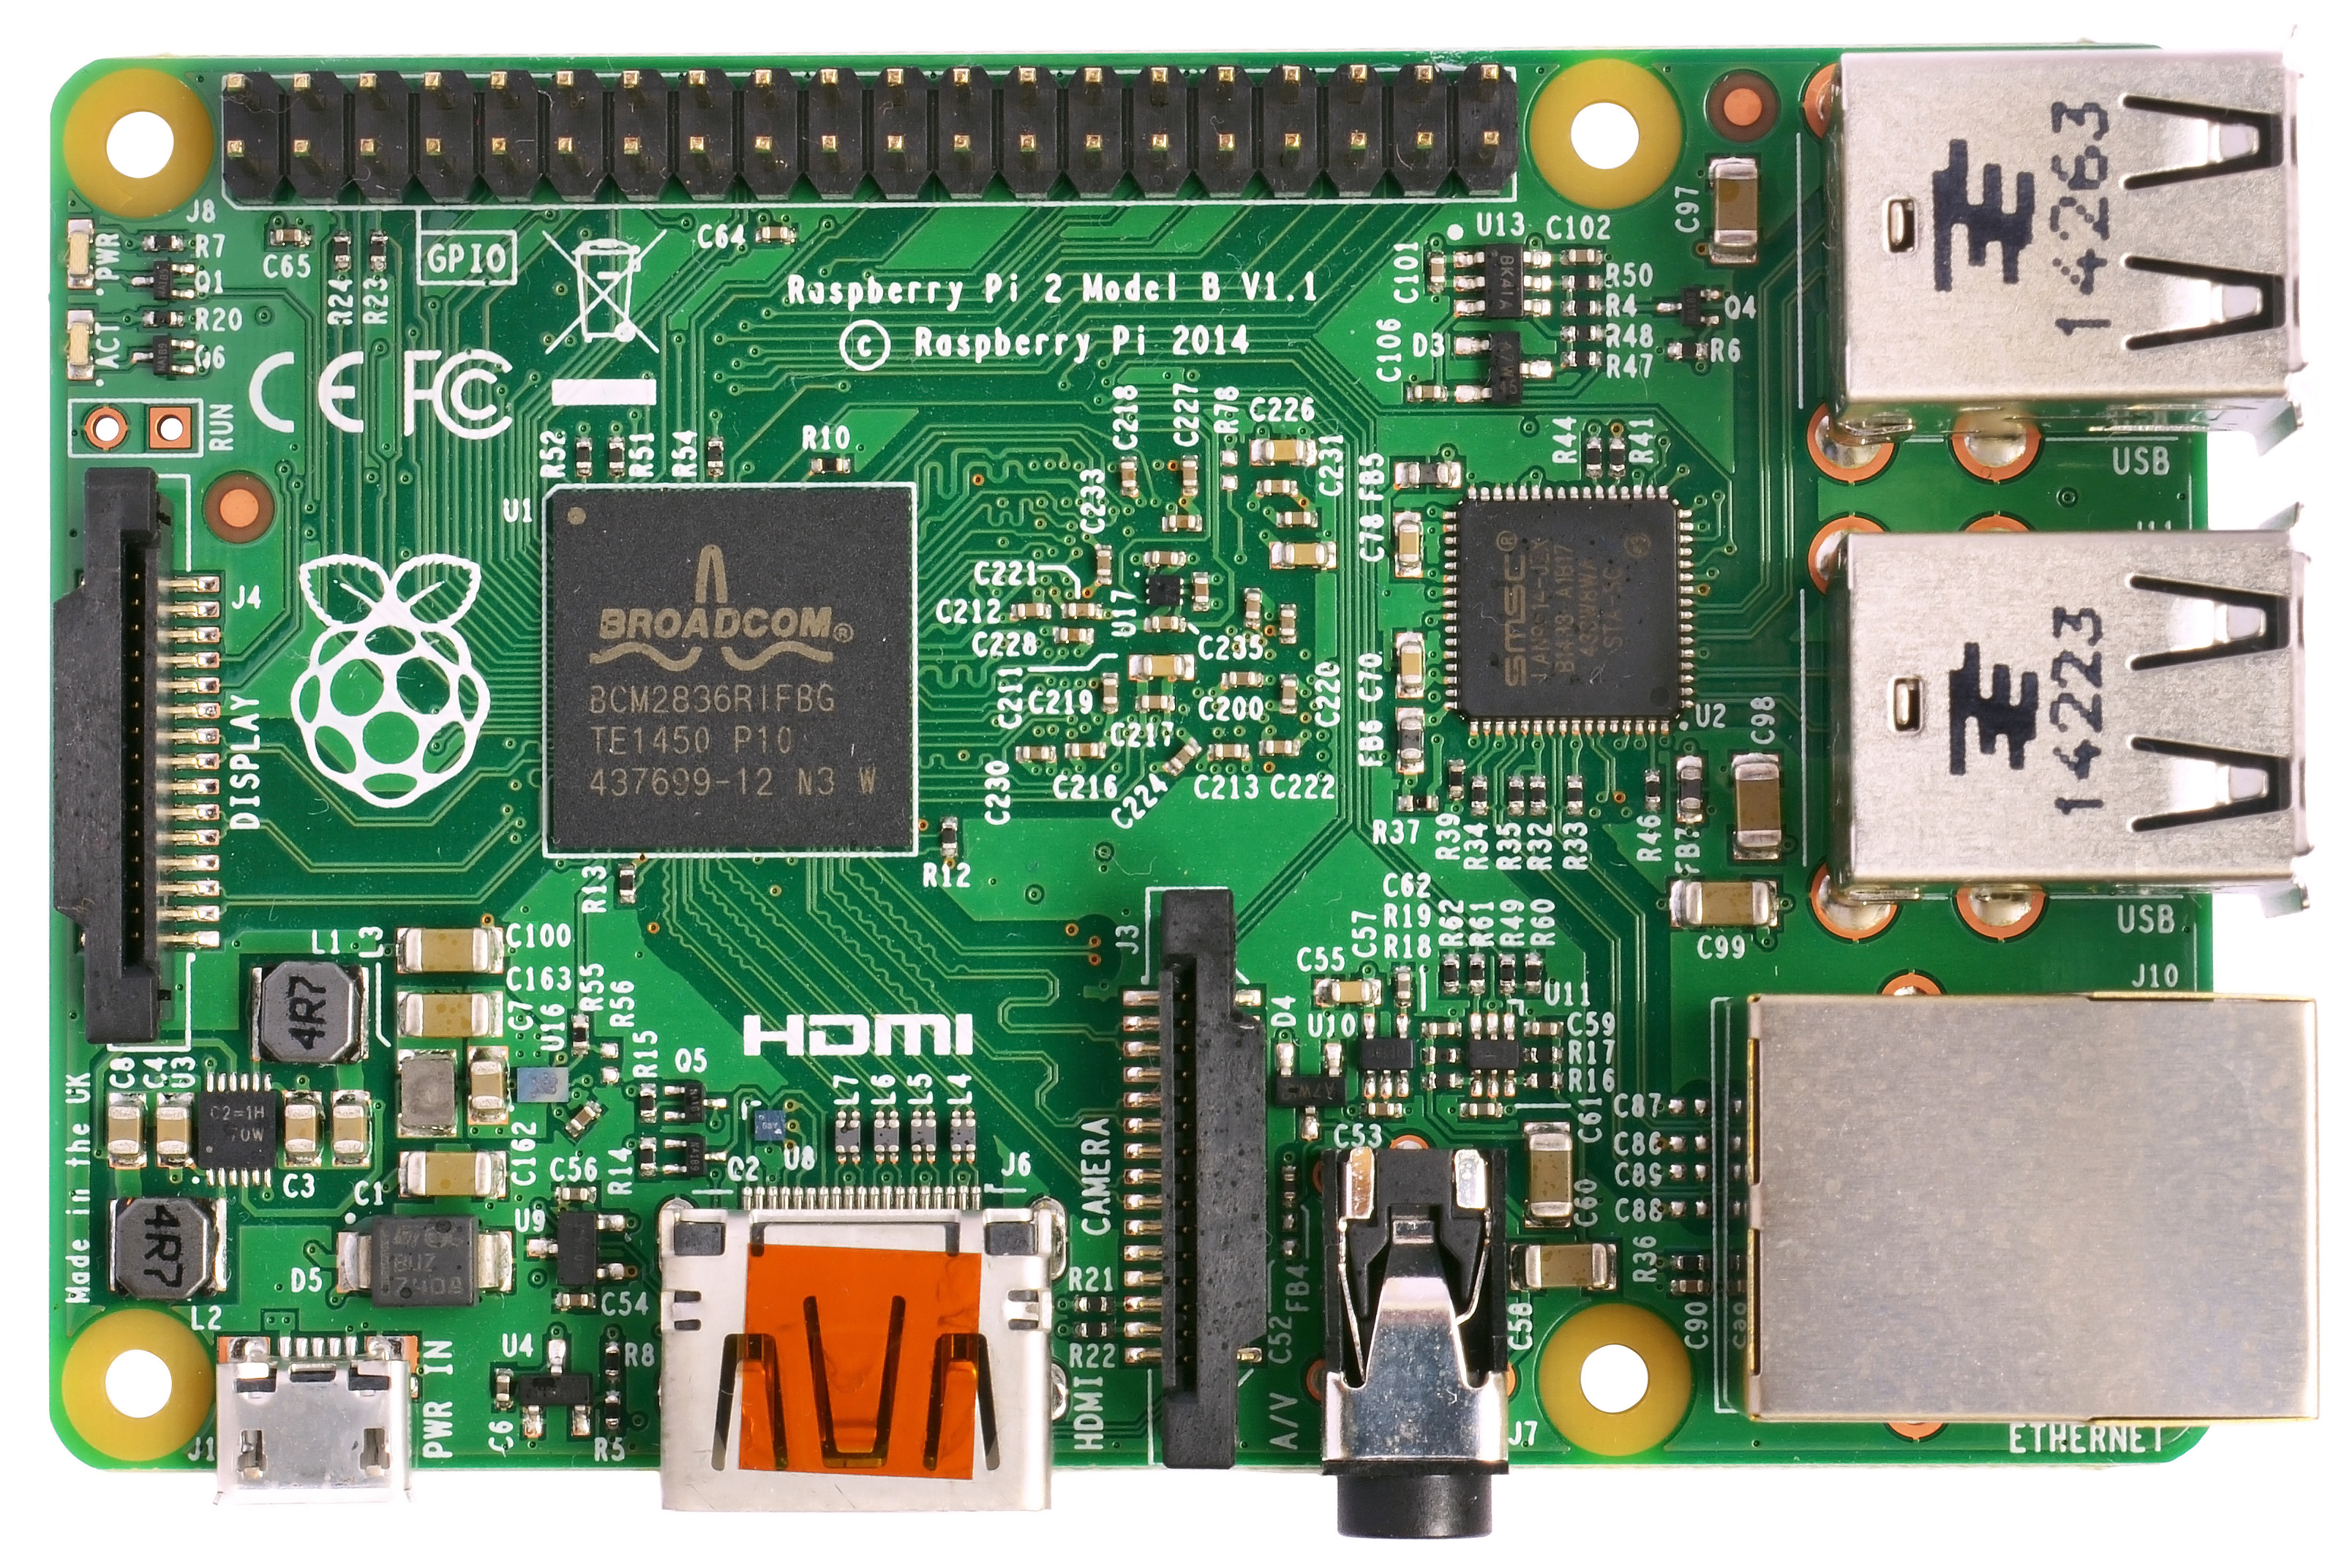
\includegraphics[scale = 0.05]{images/pi}
    \caption{A Raspberry Pi Model B.\cite{PiImage}}
    \label{fig:pi}
\end{figure}

\subsubsection{Specification}
For a full specification, it can be found on the Raspberry Pi's website
\cite{PiSpecs}.

\begin{tabular}{>{\bfseries}r l}
	System on Chip & Broadcom BCM2836 \\
	CPU & 900 MHz quad-core ARM Cortex-A7 \\
	Memory & 1 GB \\
	Ethernet (Limits) & 10/100 Mbits/s \\
	USB 2.0 & 4 Ports \\
	On Board Storage & MicroSD slot \\
	Price & £16.00 \\
\end{tabular}

\newpage

% ------------------------------------------------------------------------------
% ------------------------------------------------------------------------------

\section{Development Environment}
The development environment that we shall use for the Arduino is the Arduino
Integrated Development Environment (or Arduino Software (IDE)). For development
on the Pi we will be using Raspbian with a Java Spring application acting as our
web service for the system.

We all also be using a Git version control system in addition for easier
transferring of work between group members. For the purposes of sharing other
documents and files (for example, this report), a shared Google Drive folder was
created to allow us all to add to each other's notes with ease before being
formatted and organized properly.

The creation of the Gannt chart outlining our plan using Smartsheet, which again
allowed easy access for everyone to view progress.

% ------------------------------------------------------------------------------
% ------------------------------------------------------------------------------

\section{Additional Resources}
Note: since we felt we had relatively few additional components, we felt at this
stage a full spreadsheet would be superfluous and thus omitted.

% ------------------------------------------------------------------------------

\subsection{Coffee Pot}
Since the HTCPCP is all about sending requests for coffee, a coffee pot is
naturally required for the whole thing to work. We have decided on the Andrew
James 1100 Watt DIgital Filter Coffee Maker.

\textbf{Price}: £27.99

\textbf{Purchased from}: Amazon UK

% ------------------------------------------------------------------------------

\subsection{Barduino}
As part of our project, we have found the potential of adapting the Barduino, a
previous year’s Embedded Systems project into our own, for the use of supplying
the coffee with milk and other condiments if desired. Since the project owners
have not claimed it, it has been deemed available for appropriation.

\textbf{Price}: £0.00

\textbf{Purchased from}: N/A

% ------------------------------------------------------------------------------

\subsection{Servo Motor Controller}
\textbf{Price}: £20.50

\textbf{Purchased from}: Pimoroni
\newpage

\begin{figure}[H]
    \centering    
    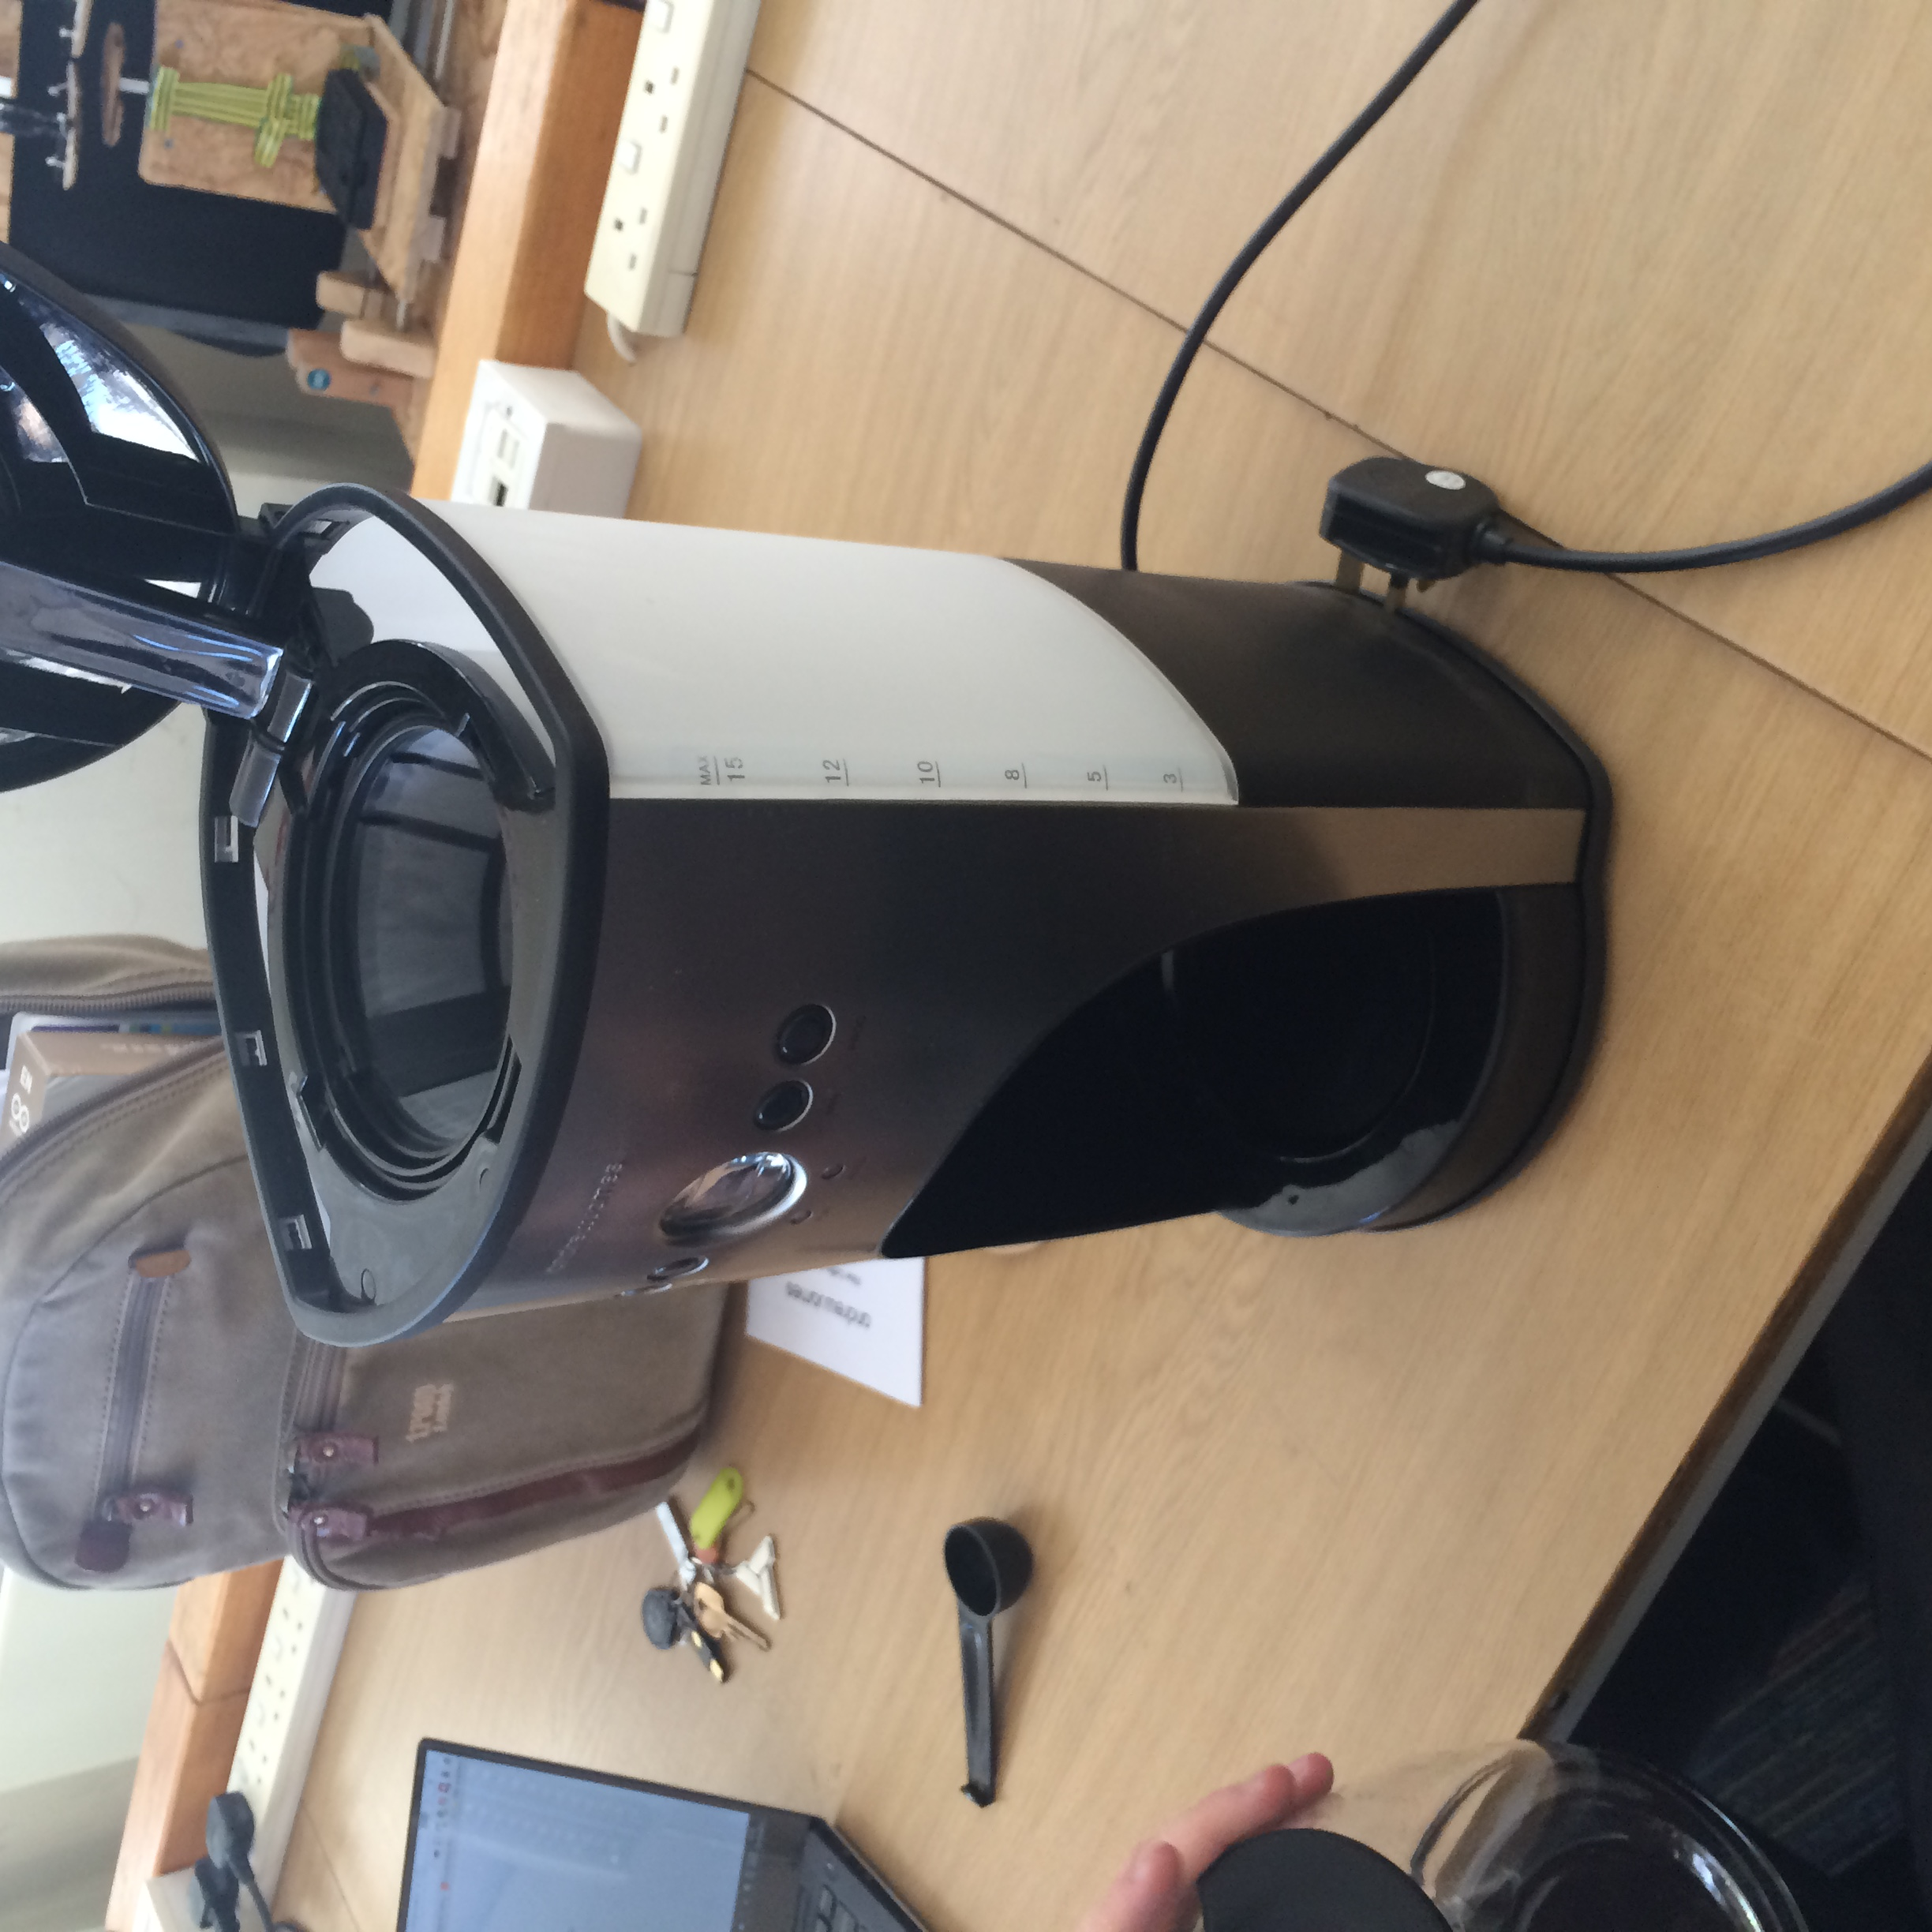
\includegraphics[height=9cm, angle=270]{images/coffee}
    \caption{The Barduino}
\end{figure}

\begin{figure}[H]
    \centering    
    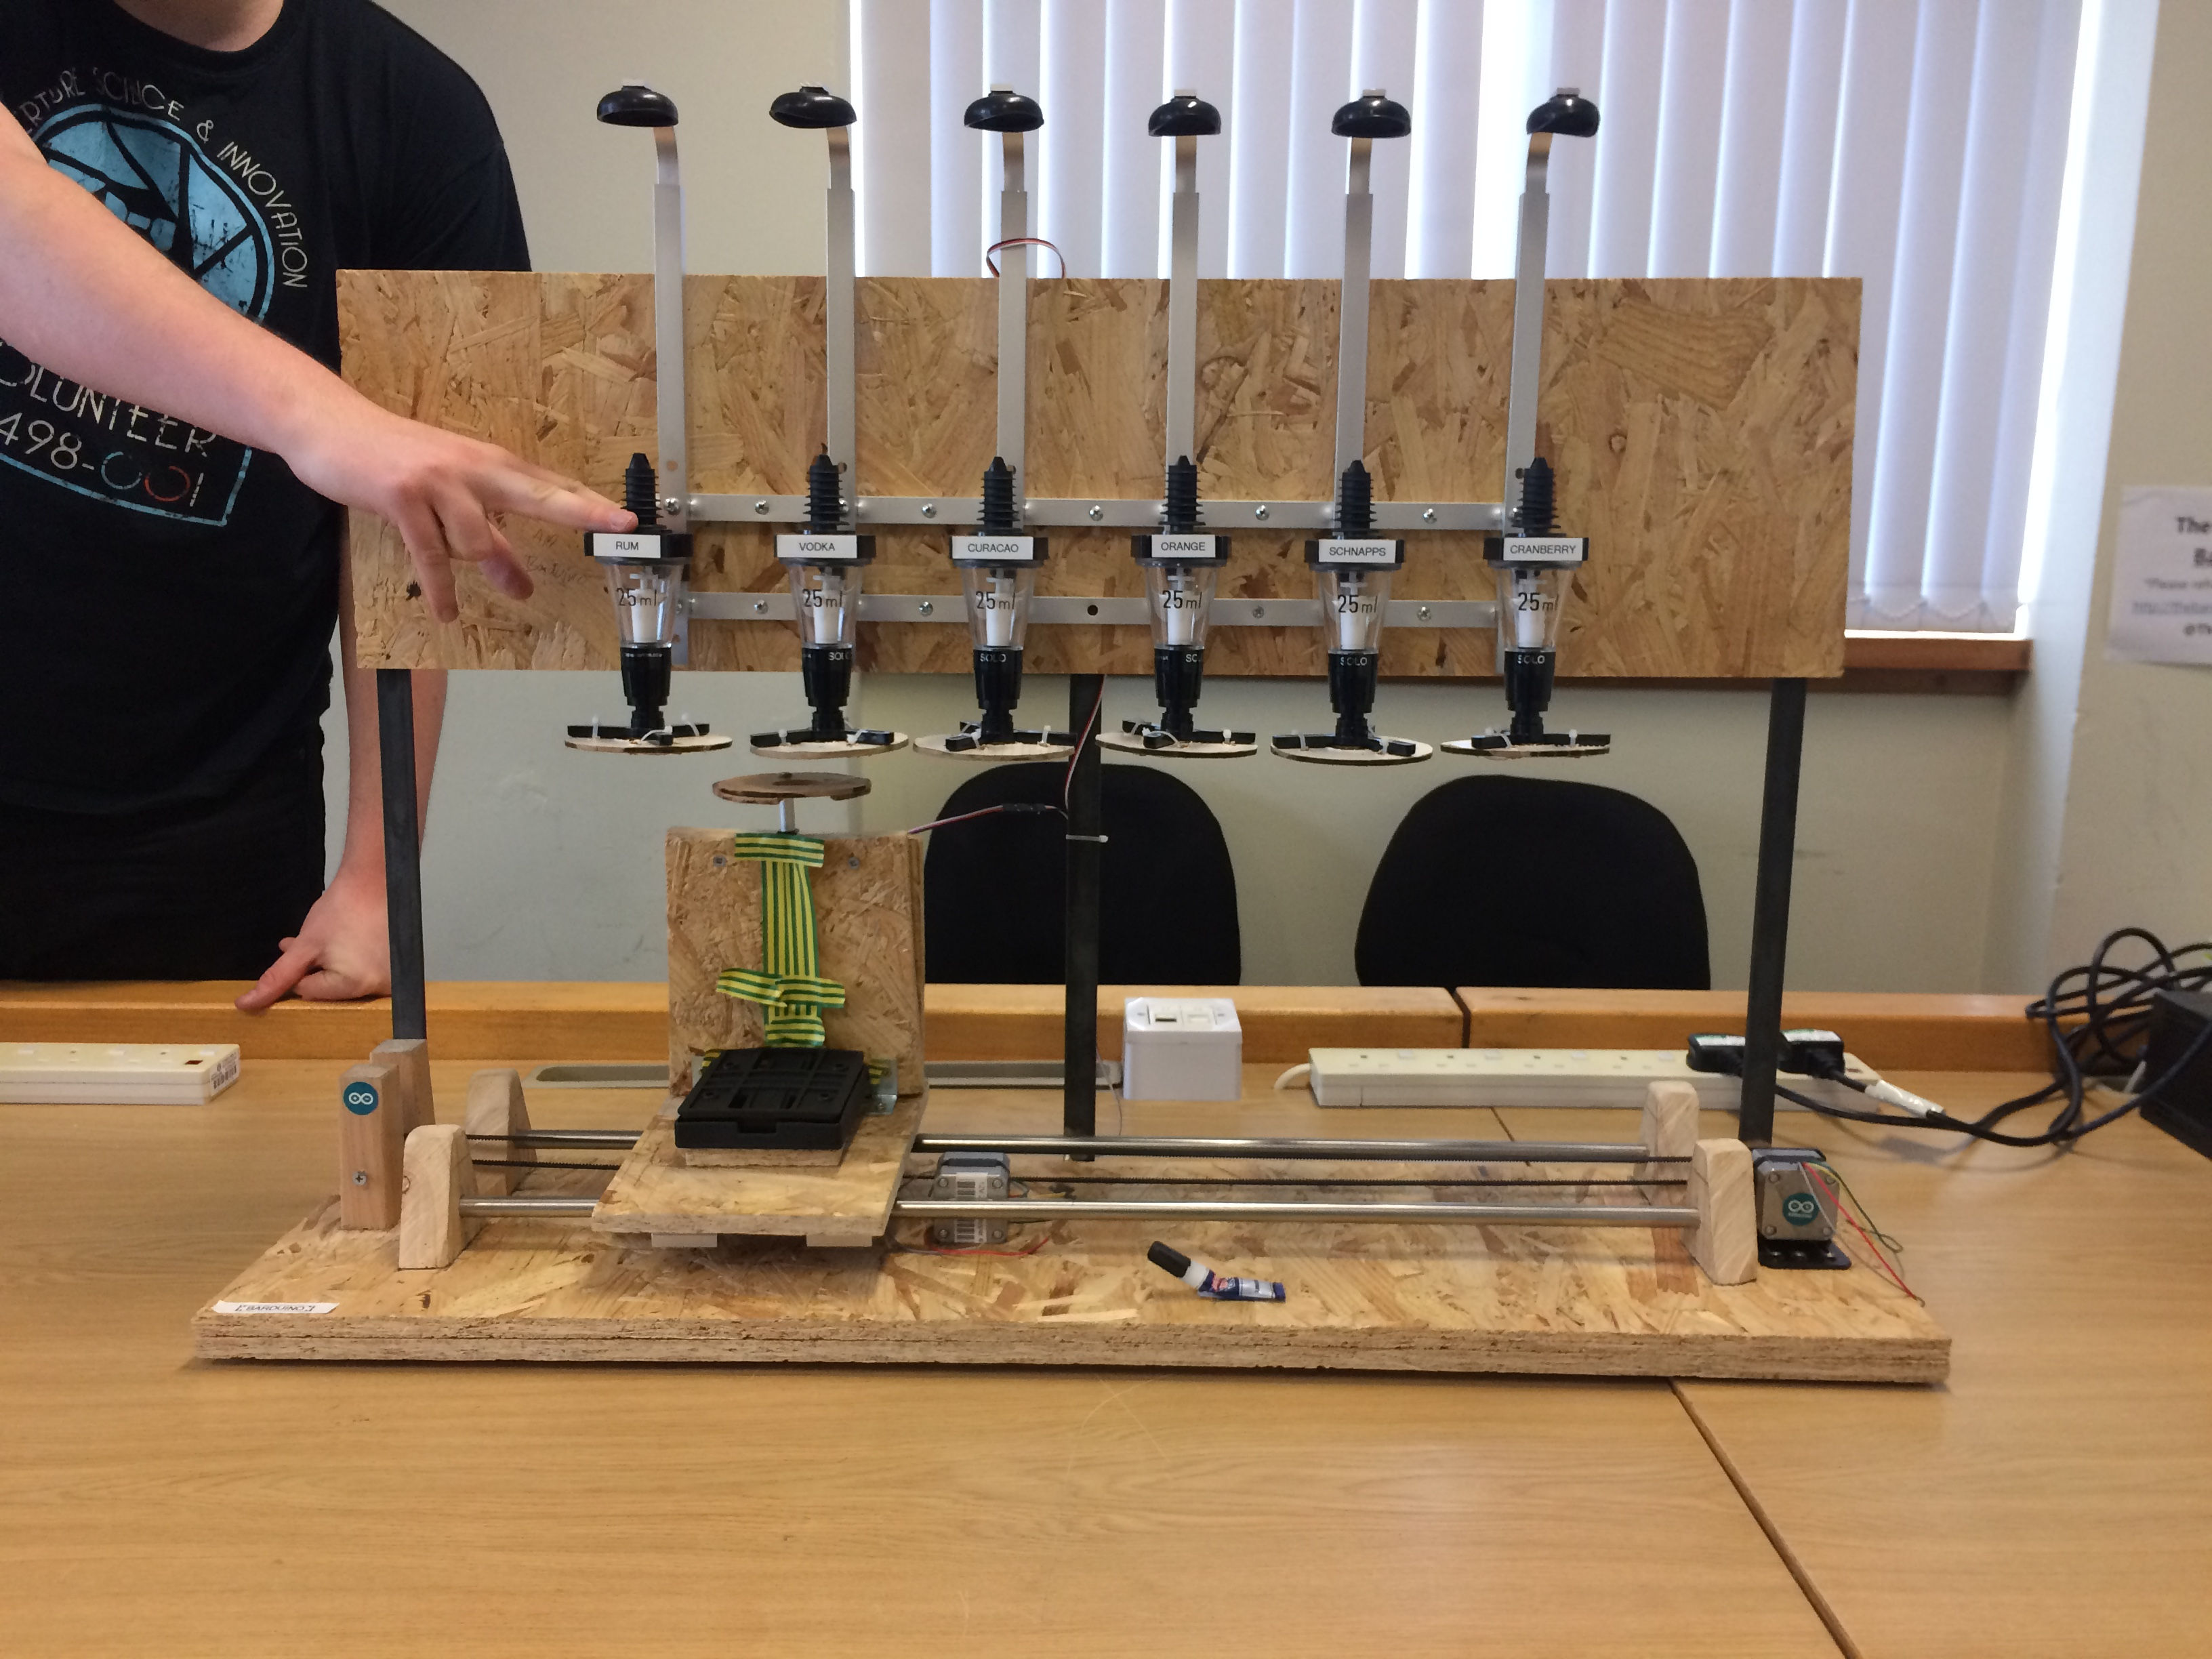
\includegraphics[height=9cm]{images/barduino}
    \caption{The Coffee Maker}
\end{figure}

% ------------------------------------------------------------------------------
% ------------------------------------------------------------------------------

\section{Planning}
A high-res version is available at:
\begin{figure}[H]
    \centering    
    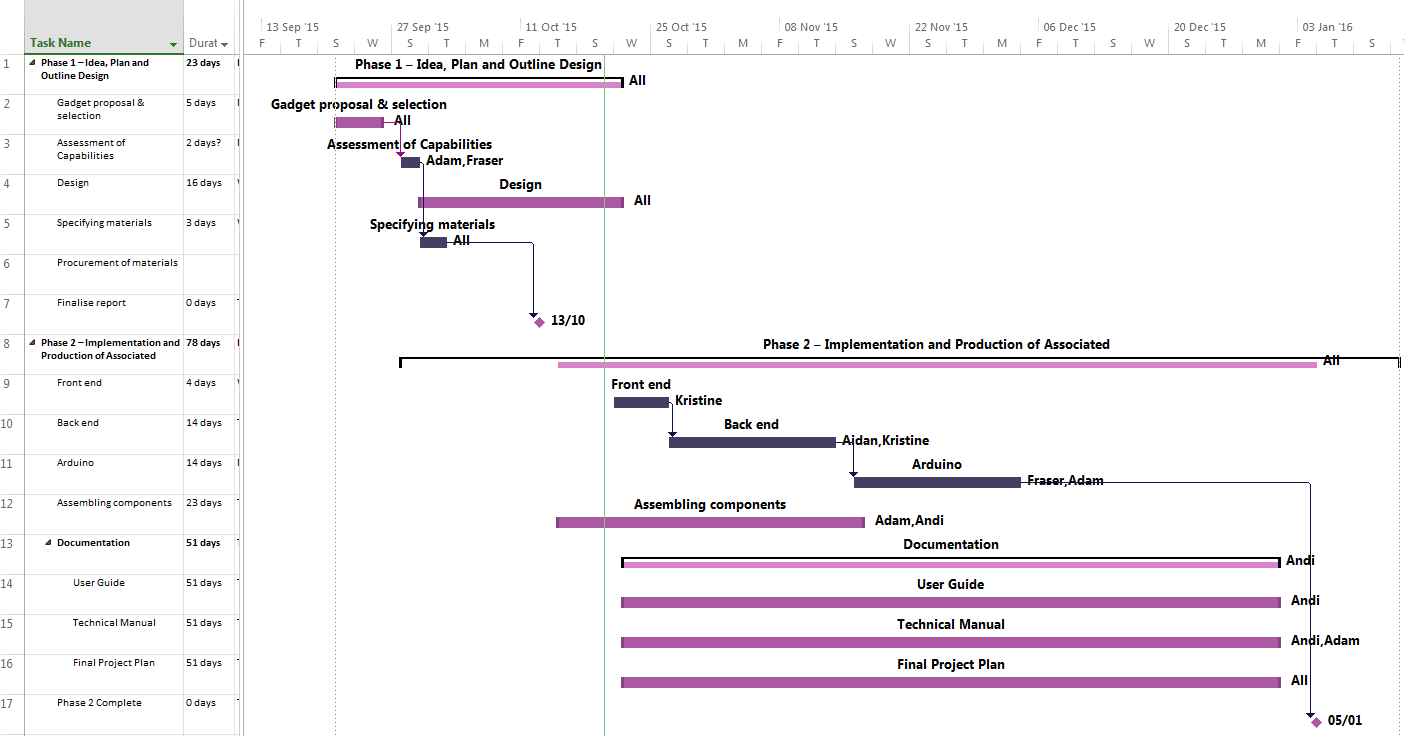
\includegraphics[angle=90, scale=0.5]{images/ProjectPlan}
\end{figure}

\newpage

% ------------------------------------------------------------------------------
% ------------------------------------------------------------------------------

\section{Design}

% ------------------------------------------------------------------------------

\subsection{Overall}
The User goes onto the Brewudino webpage (available through Pi's IP address) and 
fills out a form specifying the type of coffeee that they want. The Spring application wll recieve these requests. Accepted requests will be passed to
Arduino, which will execute code determined by the form's values.

\begin{figure}[H]
    \centering    
    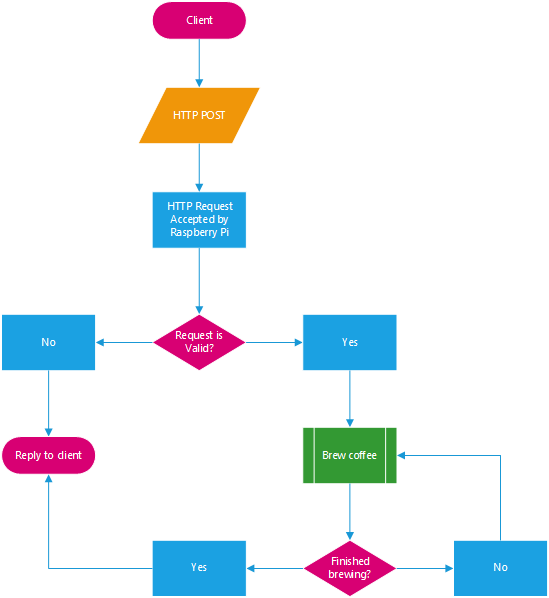
\includegraphics[scale=0.95]{images/flowchart}
    \caption{A flowchart defining how the overall system works}
\end{figure}

\newpage

% ------------------------------------------------------------------------------

\subsection{Hardware}

\newpage

% ------------------------------------------------------------------------------

\subsection{Software}
There are three primary components of the software side of this project. Those
are:
\begin{itemize}
	\item A website through which users can order coffee.
	\item A Java Spring application to handle the above requests and pass to
	Arduino.
	\item The Arduino software triggering the coffee brewing and serving.
\end{itemize}
The typical user will only be exposed to the website aspect of this stack, which
will be able to provide all neccessary information through the website, such as
when there is no coffee available.

\subsubsection{Website}
The website is relatively simple. In order to obtain coffee, all they need to
do is complete the form that is provided to them. Given the current set up, the
URL is likely to be of the form IP:8080/brewduino, where IP is the address of
the Pi. The system will ideally provide the user information such as the amount
of coffee available right now, and how many requests are currently in a queue to
be filled.

\subsubsection{Java Spring Service}
The Raspberry Pi will be hosting a Java application utilising the Spring
framework to allow for us to take the form submission and act upon it in Java.
This has the advantages of allowing communication between Java application and
the user, as well as between the application and Arduino.

The Java application is made up of four core classes, this system is a spin-off
of Spring's guide on Handling Form Submissions\cite{SpringGuide} (due to the
structure of this, a class diagram was deemed unsuitable for provision):
\begin{itemize}
	\item Application
	\begin{itemize}
		\item Main method runs the system here, through the Spring framework,
		making it an extermely simple class.
	\end{itemize}
	\item Brewduino
	\begin{itemize}
		\item This class acts a data structure representing the form the user
		fills out on the website. Each field in the class represents a part of
		the website's form.
	\end{itemize}
	\item BrewduinoController
	\begin{itemize}
		\item This class handles the requests sent from the user to the Pi, and
		acts upon them. It will validate that the input is OK, and then
		communicate with the Arduino to fulfill the request.
	\end{itemize}
	\item Arduino
	\begin{itemize}
		\item This class handles all communication with the Arduino, acting as a
		middleman between the Arduino and the BrewduinoController.
		\item The Arduino class will make use of a suitable framework, such as
		JArduino\cite{JArduino} or ZXTX\cite{RXTX} to handle communication with
		Arduino.
	\end{itemize}
\end{itemize}
\newpage

% ------------------------------------------------------------------------------
% ------------------------------------------------------------------------------

\section{Current Progress}
When we started this assignment, the Brewduino was not our original concept. The
initial idea was to create a Dalek (or Dalek like machine) whose camera could be
viewed in a browser. However, we decided to go with the Brewduino project after
it was suggested a couple of weeks later, since we felt it would be a more
interesting project to tackle. This has had the

So far, we have acquired the coffee pot and commandeered the Barduino for our
project. In addition, an early start has been made on the Spring application,
since some development was done as part of the research into its feasibility and
suitability for the Brewduino.

An attempt has been made on the disassembly of the coffee pot we are using to be
connected to our Arduino, although that has not been completed (see the plan for
the projected completion).


\newpage

\bibliographystyle{plain}
\bibliography{report} 
\end{document}